\documentclass{article}

% Language setting
% Replace `english' with e.g. `spanish' to change the document language
\usepackage[portuguese]{babel}

% Set page size and margins
% Replace `letterpaper' with `a4paper' for UK/EU standard size
\usepackage[a4paper,top=2cm,bottom=2cm,left=3cm,right=3cm,marginparwidth=1.75cm]{geometry}

% Useful packages
\usepackage{amsmath}
\usepackage{subcaption}
\usepackage{graphicx}
\usepackage[colorlinks=true, allcolors=blue]{hyperref}

\title{Trabalho Prático 02}
\author{Luciano Stork}

\begin{document}
\maketitle

\begin{abstract}
Uma vez proposta a Análise de Conjuntos Típicos e Identificação de Regiões Codificadoras em Sequências de DNA, esse relatório foi pautado no passo a passo de um projeto de pesquisa que combina a teoria da informação com a genômica objetivando utilizar conceitos de conjuntos típicos e propriedades da equipartição assintótica para identificar regiões codificadoras em sequências de DNA por meio de cálculos de entropia das sequências; identificando, assim, regiões codificadoras.

\end{abstract}

\section{Comentários Introdutórios}

Ao passo em que estão sendo explorados os principais conceitos e métodos da disciplina, vem tornando-se possível entender que o conceito de Conjuntos Típicos é fundamental para a teoria da informação, especialmente quando se trata de codificação de informações e comunicação eficiente, sendo uma parte importante na representação e na análise de sequências de símbolos em termos de conjuntos que contêm as sequências mais prováveis. Esse princípio, que tem aplicações variadas na ciência da computação e na teoria da informação, também desempenha um papel crucial na área da bioinformática, mais especificamente na Análise de Conjuntos Típicos e Identificação de Regiões Codificadoras em Sequências de DNA.

As sequências de DNA, que carregam informações genéticas essenciais para a hereditariedade e funcionamento dos organismos vivos, são constituídas por uma cadeia de quatro nucleotídeos diferentes: adenina (A), citosina (C), guanina (G) e timina (T). A ordenação precisa desses nucleotídeos na sequência do DNA é crítica para determinar as características e funções de um organismo. No entanto, em sequências de DNA de tamanho considerável, encontrar regiões de interesse, como genes ou elementos regulatórios, pode ser uma tarefa desafiadora devido à sua vastidão e complexidade.

A Análise de Conjuntos Típicos em Sequências de DNA envolve a aplicação de princípios de teoria da informação e estatística para identificar regiões altamente informativas ou significativas em uma sequência de DNA. Isso é fundamental para a identificação de genes, elementos regulatórios e outras características funcionais do genoma. A ideia central é que regiões altamente conservadas e essenciais para a função genética tendem a ser mais prováveis e, portanto, mais "típicas" em relação à composição de nucleotídeos, em comparação com regiões não funcionais ou aleatórias do DNA.

Por meio de técnicas de análise de conjuntos típicos, os bioinformaticistas podem identificar com maior precisão as regiões codificadoras que desempenham um papel fundamental na expressão gênica, na síntese de proteínas e em outras funções biológicas. Isso é crucial para a compreensão da genética e da biologia molecular, bem como para aplicações práticas, como a pesquisa médica e o desenvolvimento de terapias genéticas.

Portanto, a análise de conjuntos típicos desempenha um papel fundamental na decifração e interpretação das informações genéticas contidas nas sequências de DNA, contribuindo para avanços significativos na área da biologia molecular e da medicina, à medida que buscamos entender e manipular o código da vida de maneira mais eficaz e precisa.

\section{Desenvolvimento da Tarefa Proposta}

\subsection{Entendimento dos Conjuntos Típicos}

Para dar os primeiros passos no desenvolvimento da tarefa em questão, foi necessário entender que a Teoria dos Conjuntos Típicos é um pilar da teoria da informação que se concentra em como representar informações de forma eficiente. Ela se baseia na ideia fundamental de que, em sistemas de comunicação, algumas sequências de símbolos são mais prováveis de ocorrer do que outras. Essa probabilidade de ocorrência é usada para determinar quais sequências são consideradas "típicas" e, portanto, merecem uma representação mais eficiente. Com base nisso, surge a Propriedade da Equipartição Assintótica como uma característica central dessa teoria, estabelecendo que, à medida que o tamanho das sequências de símbolos aumenta indefinidamente, a probabilidade de uma sequência estar dentro de um conjunto típico se aproxima de 1 (indicando certeza) para a maioria das sequências. Isso significa que, na prática, podemos concentrar nossa atenção nas sequências mais prováveis e ignorar as menos prováveis com confiança. 

Na medida em que começamos a lidar com graus de certeza e confiabilidade dos resultados esperados, surge o conceito de Entropia, que torna-se reponsável por desempenhar um papel fundamental na teoria da informação. Basicamente, podemos classificá-la como uma medida de incerteza ou aleatoriedade em um conjunto de símbolos,  calculada com base na distribuição de probabilidades dos símbolos. Quanto maior a entropia, maior a incerteza. Em sistemas de comunicação, a entropia é usada para quantificar o grau de informação em uma mensagem ou sequência que, geralmente será transmitida sob a influência de algum meio de apresentação, onde surge a necessidade de explorar a Codificação como um processo de representar informações de forma eficiente. Na teoria da informação, a codificação de fonte é uma abordagem que visa reduzir a redundância em uma sequência de símbolos. Isso é feito atribuindo códigos mais curtos a símbolos mais prováveis e códigos mais longos a símbolos menos prováveis. Os conjuntos típicos ajudam a identificar quais sequências merecem códigos mais curtos, tornando a comunicação mais eficiente. 

Aliada, em uma segunda estância à Codificação, tem-se o conceito de Tamanho de Bloco, que é um parâmetro importante responsável por determinarl quantos símbolos são agrupados para formar conjuntos típicos. O tamanho de bloco influencia a eficiência da codificação e a capacidade de representar informações de maneira precisa. Escolher o tamanho de bloco apropriado é crucial para otimizar a comunicação e a compactação de dados. 

Obviamente, uma vez que estão sendo trabalhados grandes números de dados, é interessante pensar em um comportamento estatístico, e a Distribuição de Probabilidades tem papel crucial no fornecimeto de dados envolvendo as probabilidades de ocorrência de cada símbolo em uma sequência de informações. Em teoria da informação, conhecer a distribuição de probabilidades é essencial para calcular a entropia e projetar codificações eficientes. Uma distribuição de probabilidades precisa é a base para a identificação de conjuntos típicos e para a alocação de códigos.

De um modo geral, entender esses conceitos funciona como uma base para o entendimento dos Conjuntos Típicos no contexto da teoria da informação. Eles permitem que variados sistemas sejam capazes de representar informações de maneira eficiente, concentrando-se nas sequências mais prováveis, quantificando a incerteza com entropia, aplicando codificações eficientes, definindo tamanhos de bloco apropriados e utilizando distribuições de probabilidades para otimização. Certamente, essa rotina de processamento é fundamental em uma variedade de campos e áreas de atuação, incluindo a bioinformática, onde a análise de sequências de DNA e RNA depende da eficiência na representação e na identificação de informações relevantes.

\subsection{Obtenção de Sequências de DNA}

O desenvolvimento dessa prática teve como base o seequenciamento em formato FASTA da Hexokinase, uma enzima de extrema importância para os processos metabólicos em organismos vivos, com especial destaque nos seres humanos. 

Sua principal função está relacionada à glicólise, uma via metabólica central que desempenha um papel crucial na conversão da glicose, um açúcar, em unidades menores de energia, como o ATP (adenosina trifosfato). Especificamente, a hexokinase atua catalisando a primeira etapa da glicólise, onde a glicose é transformada em glicose-6-fosfato. Durante esse processo, uma molécula de ATP é consumida e convertida em ADP (adenosina difosfato). Ao mesmo tempo, a glicose é "capturada" e transformada em uma forma que não pode escapar da célula.

A escolha dessa enzima foi pautada nas possibilidades de se entender melhor como nosso corpo converte glicose em energia, um processo essencial para a sobrevivência.
Além disso, ela está diretamente envolvida na regulação dos níveis de glicose no organismo, atuando como um sensor de glicose em células do fígado e do pâncreas, contribuindo para a manutenção de seus níveis no sangue dentro de limites saudáveis. Isso é vital para prevenir condições como diabetes, em que a regulação inadequada da glicose pode causar sérios problemas de saúde.

Portanto, a exploração da hexokinase não apenas nos ajuda a compreender os processos metabólicos fundamentais que sustentam a vida, mas também é crucial para o desenvolvimento de tratamentos e estratégias de controle da glicose, melhorando assim a saúde e a qualidade de vida das pessoas.

\begin{figure}[h]
  \centering
  \begin{subfigure}{0.25\textwidth}
    \centering
    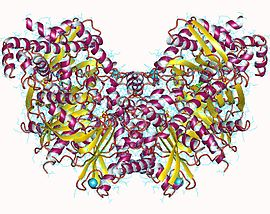
\includegraphics[width=\linewidth]{hexo1.jpg}
    \caption{\label{fig:hexo1.jpeg}Hexokinase I, dimer, Human.}
  \end{subfigure}\hspace{8em}
  \begin{subfigure}{0.25\textwidth}
    \centering
    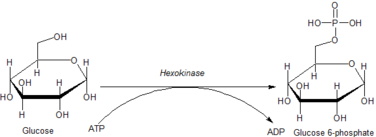
\includegraphics[width=\linewidth]{hexo2.png}
    \caption{Reação da hexoquinase com glicose como substrato}
  \end{subfigure}
  \end{figure}
  

\subsection{Cálculo da Entropia}
A Entropia de Shannon, frequentemente denotada como \(H(X)\), é calculada pela seguinte fórmula:

\begin{equation}
H(X) = -\sum_{i=1}^{n} p(x_i) \log_2(p(x_i))
\end{equation}

onde \(H(X)\) é a entropia de Shannon do conjunto de eventos  X, \(n\) é o número de eventos distintos no conjunto X, \(p(x_i)\) é a probabilidade de ocorrência do evento \(x_i\).

Considerando que essa fórmula é amplamente utilizada para medir a incerteza ou desordem em um conjunto de dados ou sistema probabilístico, é interessante que apliquemos a equação ao sequenciamento em análise para que seja calculada sua entropia, e então, seja dimensionado o grau da incerteza associada à frequência de ocorrência dos símbolos. 
Desse modo, o sequenciamento em formato FASTA da enzima Hexokinase, em sua totalidade, apresentou uma entropia \(H(X)\) igual a 2,0795.

\subsection{Identificação de Regiões Codificadoras}

Como citado anteriormente, a distribuição de entropia ao longo das sequências de DNA pode trazer informações cruciais sobre a estrutura e função do genoma. A entropia, como medida de desordem ou incerteza, desempenha um papel fundamental na caracterização da variabilidade das bases ao longo de uma sequência de DNA. Em particular, a análise da entropia pode revelar regiões de interesse dentro do genoma, especialmente quando se trata de identificar regiões codificadoras de genes.

Regiões com desvio significativo da entropia esperada podem indicar a presença de regiões codificadoras, também conhecidas como exons. Essas regiões são altamente relevantes na biologia molecular, pois representam segmentos do DNA que são transcritos em RNA mensageiro (mRNA) e, subsequentemente, traduzidos em proteínas. Devido à sua importância funcional, as regiões codificadoras tendem a exibir características distintas em termos de entropia.

É observado que as regiões codificadoras geralmente apresentam uma menor entropia quando comparadas às regiões não codificadoras, chamadas de introns. Isso ocorre devido às restrições impostas pela codificação genética. Nas regiões codificadoras, a sequência de bases é altamente conservada, o que significa que as informações nesses segmentos são críticas para a síntese correta das proteínas. A menor entropia reflete a predominância de sequências altamente específicas e conservadas nas regiões codificadoras, uma vez que as variações nesses locais podem levar a alterações nas proteínas produzidas.

Portanto, a análise da entropia ao longo das sequências de DNA não apenas fornece uma visão sobre a estrutura genômica, mas também ajuda na identificação de regiões de potencial interesse biológico. A detecção de regiões com baixa entropia pode ser um passo inicial na identificação de genes e na compreensão de como a informação genética é codificada e expressa nos organismos. 

Sintetizando as informações acima, a entropia das sequências de DNA desempenha um papel crucial na investigação e na decifração do funcionamento dos genomas, contribuindo para avanços significativos na biologia molecular e genética.

Pensando nisso, foi desenvolvida uma rotina MATLAB que começa lendo uma sequência de DNA a partir de um arquivo externo especificado pelo usuário. O nome do arquivo é definido na variável filename. Fica a cargo do usuário ajustar os parâmetros de análise, como o tamanho da janela deslizante e um limiar para identificar regiões de baixa entropia. Em seguida, o código calcula a entropia local da sequência de DNA percorrendo a sequência por meio de uma janela deslizante de tamanho especificado e, para cada janela, calcula a entropia de Shannon. Após calcular essa entropia local, são identificadas regiões de baixa entropia com base no limiar especificado. Em seguida, o código exibe as sequências de DNA que correspondem a essas regiões de baixa entropia de modo que cada sequência é acompanhada pela entropia calculada para essa sequência e pela posição na sequência original. Isso permite ao usuário visualizar as sequências com baixa entropia e entender sua localização na sequência original. Finalmente, o código cria um gráfico que representa a sequência de DNA inteira em azul e destaca as regiões de baixa entropia em vermelho. Isso fornece uma representação visual das regiões de baixa entropia na sequência.

Potanto, para elucidar a saída do código, segue um exemplo de utilização que considera a adoção de uma janela de 25 símbolos e um limiar de decisão de 1,5.

\begin{figure}[h]
  \centering
  \begin{subfigure}{0.5\textwidth}
    \centering
    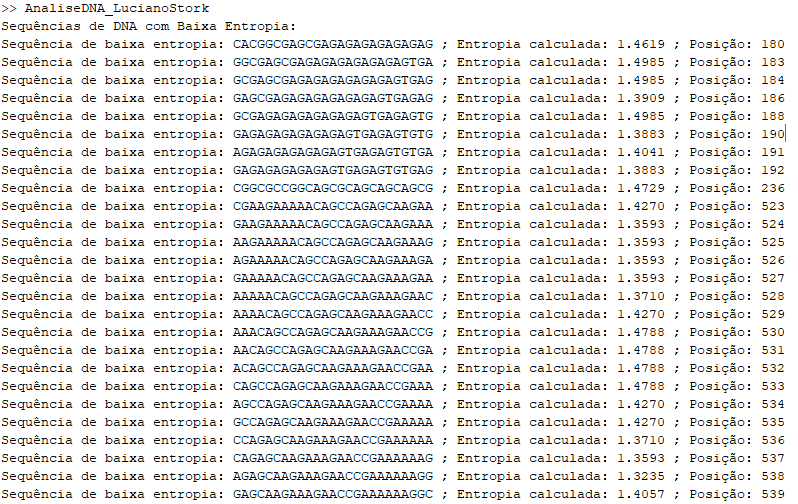
\includegraphics[width=\linewidth]{Cod1.png}
    \caption{\label{fig:hexo1.jpeg}Regiões de baixa entropia}
  \end{subfigure}\hspace{8em}
  \begin{subfigure}{0.5\textwidth}
    \centering
    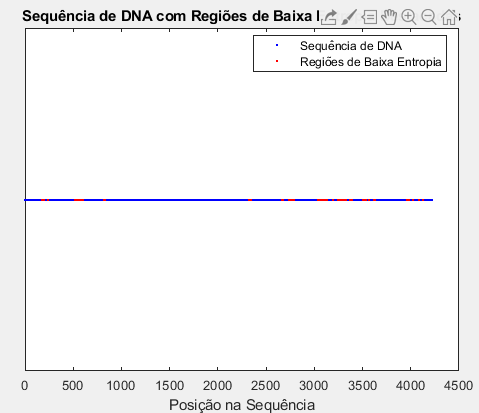
\includegraphics[width=\linewidth]{Cod2.png}
    \caption{Apresentação visual da sequência}
  \end{subfigure}
  \end{figure}
  


\subsection{Validação Experimental}
Levando em consideração a complexidade dos estudos que associam os conceitos da teoria da informação aos paradigmas genômicos, não é uma tarefa trivial encontrar informações que interligam os assuntos e os relacionam de forma prática e acessível a ponto de servirem como base de estudo e comparação de resultados, sobretudo quando focamos nossa atenção a uma cultura específica, no nosso caso, da Hexokinase. Desse modo, seria aconselhável buscar fontes acadêmicas confiáveis, como pesquisas relacionadas à Hexokinase e à teoria da informação aplicada à genômica, ou ainda  entrar em contato com especialistas na área para, de fato, validar o método comparando-o a resultados técnicos experimentais.

No entanto, a nível de um trabalho prático, os resultados apresentam certo grau de confiabilidade em função da assertividade de implementação do código, que foi testado para outras informações das quais se tem um gabarito de verificação. 

Outra forma de verificação é por meio da comparação com bancos de dados de genes conhecidos, como o GenBank. Lá, é possível encontrar informações sobre a sequência de DNA em estudo, sendo possível verificar a validade das regiões codificadoras identificadas.

\section{Conclusões}
Com base na execução do referido trabalho prático, torna-se evidente a importância dos conceitos da teoria da informação para que seja possível extrair informações importantes não só da própria área da comunicação digital, como é explorado nas questões envolvendo codificação e análise das transmissões de informações, mas também nos outros diversos cenários e aplicações do desenvolvimento humano. Como visto, a análise genômica por meio da diferenciação das sequências a partir da variação da entropia abre um vasto leque de oportunidades para a compreensão e manipulação do código genético.

Nesse contexto, a teoria da informação revela-se uma ferramenta crucial para decifrar os segredos do DNA, uma vez que a variação da entropia nas sequências genômicas pode revelar padrões, mutações e informações funcionais fundamentais para a biologia e medicina. A habilidade de quantificar a complexidade e a incerteza nos dados genéticos permite não apenas uma compreensão mais profunda da evolução e da diversidade da vida, mas também o desenvolvimento de terapias personalizadas, a identificação de predisposições genéticas a doenças e o avanço da pesquisa biomédica como um todo.

Além disso, essa abordagem não se restringe apenas ao âmbito da genômica. Os princípios da teoria da informação podem ser aplicados em áreas tão diversas quanto a análise de dados financeiros, o processamento de linguagem natural, a otimização de redes de comunicação e a tomada de decisões em situações complexas. Assim, a integração dos conceitos da teoria da informação em diferentes disciplinas e campos de estudo representa um caminho promissor para desvendar e aproveitar o potencial da informação em suas várias formas.

Em resumo, a análise genômica e a exploração da variação da entropia exemplificam como a teoria da informação transcende as fronteiras tradicionais e se insere como uma base sólida para a compreensão e o progresso em inúmeras áreas do conhecimento e da tecnologia. É evidente que a aplicação desses princípios continuará a desempenhar um papel fundamental na expansão do nosso entendimento do mundo e na melhoria das nossas capacidades em moldar o futuro.

Cabe citar, entretanto, que é de suma importância que o operador identifique e saiba dimensionar a parametrização na aplicação dos conceitos da teoria da informação de modo a extrair as informações necessárias, evitando que sejam obtidos dados enganosos, decorrentes de abordagens inadequadas na análise; ou mesmo que as informações mais relevantes sejam obscurecidas devido a orientações equivocadas. 

No experimento em questão, o código que identifica as regiões codificadoras é snsível a basicamente dois parâmetros: o \textbf{Tamanho da Janela} e o \textbf{Limiar de baixa entropia}. Desse modo, o ajuste equivocado desses fatores pode comprometer drasticamente o resultado da pesquisa.Seguem, abaixo, imagens referentes às alterações no Tamanho da Janela de análise:

\begin{figure}[h]
  \centering
  \begin{subfigure}{0.20\textwidth}
    \centering
    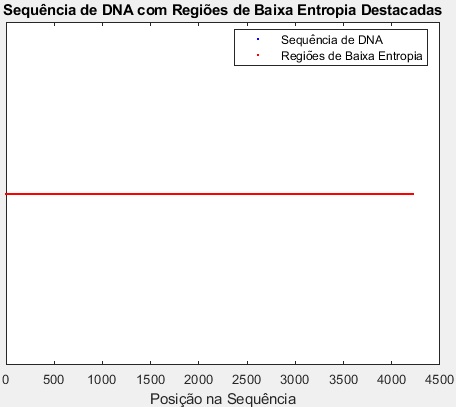
\includegraphics[width=\linewidth]{Janela1.png}
    \caption{1 símbolo }
  \end{subfigure}\hspace{1em}
  \begin{subfigure}{0.20\textwidth}
    \centering
    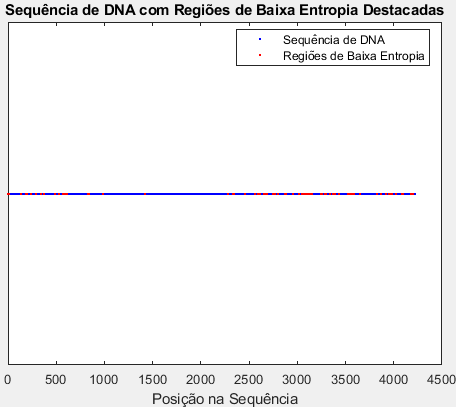
\includegraphics[width=\linewidth]{Janela10.png}
    \caption{10 símbolos}
  \end{subfigure}\hspace{1em}
  \begin{subfigure}{0.20\textwidth}
    \centering
    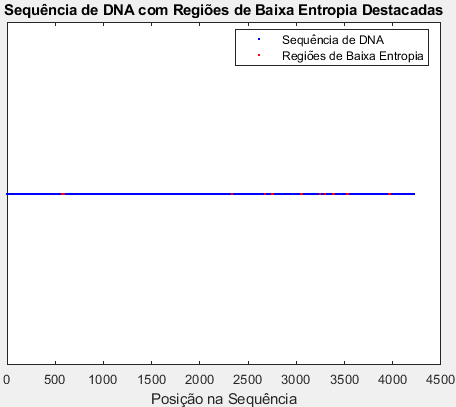
\includegraphics[width=\linewidth]{Janela20.png}
    \caption{20 símbolos}
  \end{subfigure}\hspace{1em}
  \begin{subfigure}{0.20\textwidth}
    \centering
    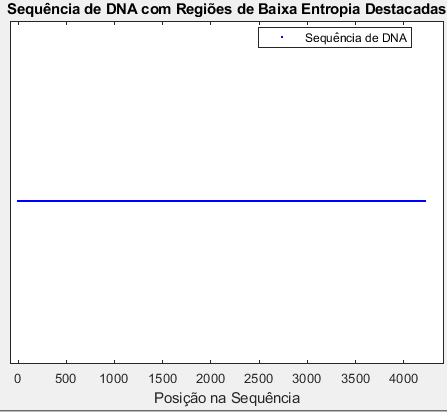
\includegraphics[width=\linewidth]{Janela50.png}
    \caption{50 símbolos}
  \end{subfigure}
  \end{figure}

Com base na análise dessas figuras, torna-se notório que  a escolha do tamanho da janela no código pode afetar como as informações são agrupadas, de modo que um tamanho de janela maior pode agrupar mais informações em um único cálculo de entropia, enquanto um tamanho de janela menor pode dividir as informações em segmentos menores. Dessa forma, se a janela for muito grande, pode haver uma perda de detalhes nas regiões de alta entropia. Por outro lado, se o tamanho da janela for muito pequeno, pode ser difícil identificar regiões de baixa entropia com precisão.

Assim percebido, nota-se que para sequências curtas, o modelo de grande número de eventos raros não se aplica. Ao crescer o comprimento das sequências analisadas, observa-se a lei de Zipf, em que algumas características (ou sequências de nucleotídeos) são muito mais comuns do que outras. Isso significa que certos elementos ocorrem com alta frequência, enquanto a maioria dos elementos ocorre com baixa frequência. Já para sequências muito longas, a PEA passa a ser preponderante, assumindo que, com um conjunto de dados geneticamente grande o suficiente, todas as sequências de nucleotídeos terão frequências aproximadamente iguais. Isso significa que, à medida que a sequência genômica se torna muito extensa, a distribuição de frequência se aproxima da equipartição, onde todas as sequências são igualmente frequentes.


\bibliographystyle{alpha}
\bibliography{sample}
\begin{enumerate}
    \item https://en.wikipedia.org/wiki/Hexokinase
    \item https://www.sciencedirect.com/topics/biochemistry-genetics-and-molecular-biology/hexokinase
    \item https://www.sciencedirect.com/topics/earth-and-planetary-sciences/hexokinase
    \item https://proteopedia.org/wiki/index.php/Hexokinase
    \item https://www.ebi.ac.uk/interpro/entry/InterPro/IPR022672/
    \item https://www.ncbi.nlm.nih.gov/pmc/articles/PMC4291497/
    
\end{enumerate}
\end{document}